\chapter{Ionisation et excitations}
\section{Introduction}
Les ionisations produites par des particules chargées jouent un rôle fondamental dans le principe
de détection. Dans les solides et les gaz on produira une parie d'électrons et d'ions positif suite
à l'ionisation d'atomes tandis que dans certains solides on créera une paire électron-trou. Dans
les deux cas, on parlera de \textbf{paires d'ions}.\\

Les électrons et ions créés par la particule chargée incidente sont les ionisations primaires mais
si ces électrons ont assez d'énergies ils peuvent aussi ioniser et causer des ionisations secondaires.

\section{Ionisation dans les gaz}%sl5
L'énergie perdue par la particule chargée traversant un gaz est répartie entre deux types 
d'interaction
\begin{enumerate}
\item \textit{L'ionisation} : un ou plusieurs électrons sont arrachés de l'atome
\item \textit{L'excitation} : l'atome est amené dans un état excité sans création d'une paire d'ions
\end{enumerate}\ 

Même si $\sigma_i>\sigma_{ex}$, le processus d'excitation domine le plus souvent car les collisions
avec faible transfert d'énergie sont les plus probables et l'énergie d'ionisation est supérieure à 
l'énergie d'excitation.

\subsection{Détermination de $W$}%sl7
L'énergie moyenne $W$ déposée par paire ion-électron formée est donnée par (c'est \textbf{la} valeur 
importante)
\begin{equation}
W=\frac{E_{abs}}{N_i}
\end{equation}
où $E_{abs}$ est l'énergie perdue par la particule incidente et $N_i$ le nombre de paires formées
sur l'ensemble de la trajectoire de la particule. Si la particule incidente est stoppée dans le 
milieu, $E_{abs}=E$. Nous avons aussi que $W>E_i$ car une partie de l'énergie est perdue via les
excitations.\\

Il est très hasardeux de se lancer dans le calcul précis de $W$ car si la section efficace considérée
est fausse, le calcul le sera aussi. Et comme l'expression de la section efficace est méconnue\dots
Il va donc falloir ruser. Si la particule chargée est totalement stoppée dans le gaz
\begin{equation}
E=N_i\langle E_i\rangle +N_{ex}\langle E_{ex}\rangle+N_i\langle \epsilon\rangle
\end{equation}
où $N_i$ est le nombre de paires produites, $N_{ex}$ le nombre d'excitation produites, $E_i$ 
l'énergie d'ionisation, $E_{ex}$ l'énergie moyenne pour créer une excitation et $\epsilon$, 
l'énergie moyenne des électrons dont l'énergie est inférieure à l'énergie d'excitation 
(électrons de sous-excitation).\\

Les électrons de sous-excitation sont les électrons dont l'énergie est insuffisante que pour 
produire des atomes excités (et donc aussi des ionisations). Ils sont importants car c'est eux
qui sont mesurés en constituant le courant d'ionisation. Leurs nombre correspond au nombre d'ions
et donc au nombre de paires $(N_i)$ par conservation de la charge électrique totale. En effet, 
tôt ou tard, après avoir perdu plus ou moins d'énergie, un électron deviendra un électron de 
sous-excitation car l'énergie d'un électron ne peut pas arriver à zéro. \\

Dans l'expression de $W$, tous les termes dépendent de $E$. Cependant, si $E\gg I$, cette 
dépendance est faible. Peu de calculs théoriques ont été fait à part pour l'hélium. En 
général, $W$ est déterminé expérimentalement (pour un gaz, $W\approx 30$ eV).

\subsection{Mélange de gaz}
Ajouter une faible quantité de certains gaz à un gaz noble augmente fortement le nombre d'ionisations
crées. Cet effet à tendance à se produire aux faibles concentration de gaz ajouté et est d'autant plus
important que le potentiel d'ionisation du gaz ajouté est petit par rapport à l'énergie de liaison des 
premiers états excités du gaz noble. La collision d'un atome excité du gaz noble avec une molécule
ajoutée peut conduire à l'ionisation de celle-ci. On utilise donc toujours des mélanges de gaz 
en pratique, l'idée c'est vraiment que cela permet d'augmenter $W$.


\section{Ionisation dans les solides}%sl15
	\begin{wrapfigure}[7]{r}{3.7cm}
	\vspace{-15mm}
	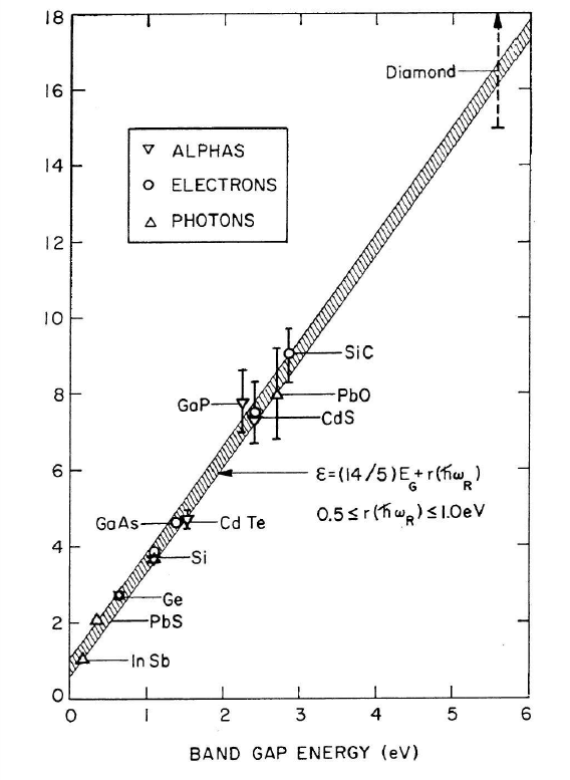
\includegraphics[scale=0.25]{ch6/image1}
	\captionof{figure}{ }
	\end{wrapfigure}
Dans les semi-conducteurs, il se forme une paire électron-trou. L'énergie pour former cette paire
est bien plus faible que pour les gaz : elle correspond au gap, de l'ordre d'1 eV. Le processus
d'excitation cause ici la création de phonons d'une énergie approximativement 0.04 eV (60\% de
l'énergie déposée donne lieu à l'excitation de phonons). Le facteur de production de paire entre
un SC et un gaz est d'à peu près 10. On constate que $W>E_g$ mais que $W/E_g$ est à peu près 
constant pour tous les SC.

\subsection{Fluctuation du nombre d'ionisation}
La fluctuation du nombre d'ionisation étant importante (limite la précision de la mesure de 
l'énergie à partir de $N_i$), il faut connaître la statistique de $N_i$ . On sait que sa valeur
moyenne vaut $N_i=E/W$. La variance $\sigma_i^2$ caractérise ces fluctuations. Considérons deux
cas extrêmes
\begin{enumerate}
\item Le nombre d'ionisation obéit à une loi de \textsc{Poisson} : la variance est la moyenne $
\sigma_i^2=N_i$.
\item Une fraction fixe de l'énergie de la particule est convertie en ionisations : c'est parfait, 
il n'y a pas d'oscillation $\sigma_i^2=0$.
\end{enumerate}\ 

La réalité se situe bien évidemment entre les deux (toutes les créations de paires ne sont pas
indépendantes)
\begin{equation}
\sigma_i^2 = FN_i
\end{equation}
où $F$ est le facteur de \textsc{Fano} tel que $0<F<1$.

\section{Facteur de Fano}
Ce facteur $F$ contient toutes les différences entre la réalité et la statistique de 
\textsc{Poisson}. Il dépend de manière détaillée de la succession des événements conduisant à la
création de paires mais c'est quasiment impossible de le déterminer théoriquement : il est
\textbf{toujours} obtenu expérimentalement.